\documentclass[12pt]{article}

\usepackage[margin=1in]{geometry}
\usepackage{amssymb}
\usepackage{amsmath}
\usepackage{graphicx}
\usepackage{subcaption}
\usepackage{cleveref}       % this package must be loaded at the last

\setlength{\parskip}{1em}
\setlength\parindent{0pt}

\newenvironment{question}[2][Question]{\begin{trivlist}
\kern10pt
\item[\hskip \labelsep {\bfseries #1}\hskip \labelsep {\bfseries #2.}]}{\end{trivlist}}


\begin{document}

\title{DD2424 Deep Learning in Data Science Assignment 4}
\author{Lin Chun Hung, chlin3@kth.se}

\maketitle

\section{Basic Part (Part 1)}

\begin{question}{i}
I used the central difference method to calculate the numerical gradients
with respect to all the network parameters and used it check against with the
analytical gradients.

I checked the maximum relative error which was mentioned in assignment and I 
used the numpy function \texttt{numpy.testing.assert\_allclose} to test if 
the gradients calculated analytically and numerically are closed element-wise.
During this time, the RNN model was set to be calculated in double precision. 

For the maximum relative error, only the \texttt{grad\_output\_wgt} went up to 
0.033. I think it is okay as the numerical gradient is calculate after the non-linear
activation layer. Other gradient maximum relative errors are pretty low and 
which are expected.

For the test assertion, consider the following equation:
\begin{equation*}
    % absolute(a - b) <= (atol + rtol * absolute(b))
    |a - b| \leq (\texttt{atol} + \texttt{rtol} * |b|)
\end{equation*}
where \texttt{atol} and \texttt{rtol} are the tolerance parameters.
In the assertion, I set \texttt{atol} to be 1e-3 and \texttt{rtol} to be 1e-4.

With these checking, I considered my analytical gradient calculations were bug free.
\end{question}

\begin{question}{ii}
I ran the training for 10 epochs, the smooth function is plotted in 
\cref{plt:smooth_lost_basic_rnn}.

\begin{figure}[h]
    \centering
    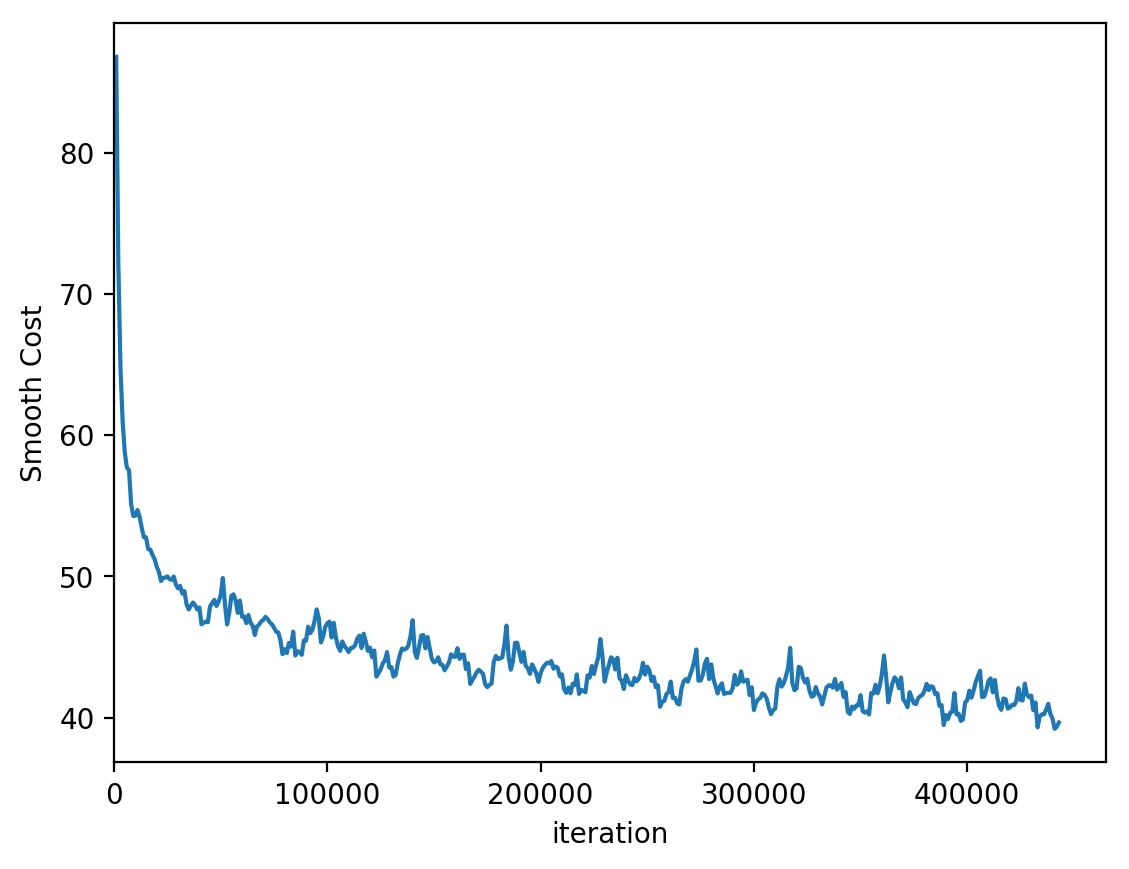
\includegraphics[width=0.8\textwidth]{./basic_cost.png}
    \caption{The smooth loss function plot}
    \label{plt:smooth_lost_basic_rnn}
\end{figure}
\end{question}

\begin{question}{iii}
The evolution of the text synthesized by the RNN:

\textbf{Iteration: 10000; smooth\_loss: 54.300842}

wadl't no oflen and Taroum sarr.  Arin ioBs tow?"
"Ave sbeks,e at cave yot lofm it wrat?"
Many, ckoary't no Slagkack, ds thamy Hurly, "Haulce to trom, wald riteraig Han. i coy.
"Goch bepny him she wav

\textbf{Iteration: 20000; smooth\_loss: 50.695659} 

Thar of thenenom in goor Rin piak beest mlemtiresease bicwing got at tle Doresjrofiro he to haillonked to bugance ald the lakK 'ilk, tor it inch Hiriaged, Kigon lecroke they rint and we ewaks'ch?"  bi

\textbf{Iteration: 30000; smooth\_loss: 49.151183} 

the groungerfirts was or the waider.  Harryd eee, was astid. . . baigagck in the reed over and of thoum!  Therimelnf.  Tall and hild.  "Harry . rars, sapkemas gevery prapur, as wis her sqommed firmirg

\textbf{Iteration: 40000; smooth\_loss: 47.801218} 

o wasce there Vortirn pawling od in thaigwan or and Harry.
"Vored; his werr tnew he iss foreracted and were in Vlasese'ld my cherered at with his his fundonarory him thing not eetrll was refave the tr

\textbf{Iteration: 50000; smooth\_loss: 48.678799} 

tent, thoughanced vidsd may hach Hamoud the's that --Ee pletis anychurgyefve Magisuply.  Impley.  "Yourceuch.
"Peveryston oncauspost of that it sulls of any wiou bemave acroutivitcyed paidy havily Pat

\textbf{Iteration: 60000; smooth\_loss: 47.148582} 

rgalne.
"Fumparit!" Harry tan to Harry stald lose.
"It preven-was tose."
"We she arst's wadlt and Heachy -"Weed.
"A. A the sping be abatame werted a plaginy. .
"a dor had to sableelans th''d," said Ro

\textbf{Iteration: 70000; smooth\_loss: 46.919232} 
, deally chom had in ooplem.
"Os the cou?" She Monef he and oge he hee cey, whon stane sevit lak. . . and on goone and sabcint to fidged, they about dobnew, and Hewilked had but hall.
Hedenter.  An th


\textbf{Iteration: 80000; smooth\_loss: 44.844659} 
d murn grene - id acrinsine, his awo out of and the laring aly.  Aed In, soke wantortaring tood suromet was ever ioned of seak had en bestroffinifn dich witutridatled to ky spatce arynont Daghstat out

\textbf{Iteration: 90000; smooth\_loss: 45.451136}

 his the stolling of them arust colmses fomfan or yow is him?  Who cool sture a magrinh," said you?  Haw light and the prot us mowaristry Mongiaperion, wion his the ame in.  Aid to be keevery an they 


\textbf{Iteration: 100000; smooth\_loss: 46.684593} 

o wandore conk look-was a douming a mound?  The ruw wefare all.  "Harry, the wand, though behc of heenbales ceely was himly rakeny out in squttin a mile, badey, to way excrow and is dighter, Hermione 

\end{question}

\begin{question}{iv}
The synthesized text after 443000 iterations is below. The smooth loss at that time is 39.663490.

He was once.  He graz and yoth was even to pould"  say deall shwioly lite expents; Harry. Harry on dear come it!  The Dumbagentruck.  The Boaked looking underilte, Aven' Maside, Harry well thombled had to the tels," situper.
"But they wort mumportobstly from Harry, "It looked term yame to Sillely wisted said.  Harry "
On turncerce-diss was sturt half lebreass know diald Mad mosted the fourg, and puice."
Hogwarts to to tre contirain farol to hair to looked said, "I do. Hare a ed, all I lew head gming he'd alause him."
It have it, the ground, wack.  Harry sausess his in and Dumbledore point!"  he on, that the good hands exan mauth . . . slise, fan as his feet casped, he the mast gowl about light imared he come comintith, about too that then, reen everner.  Horry and fater, hee I knew.  I wand."
"I ser as faur to re flear, to giin!" said.
Dagwersin blessoyed conize his Cequaching two eudley,
Harry rette Cnotha that you the question,"
Harrke it apprath.  He Poldentcimated.
"You was it me

\end{question}

\section{Optional Part (Part 2)}

For this section, I added a filtering class to help me filtering some text.
The filtering class is for:

\begin{enumerate}
    \item  Remove the URLs
    \item  Remove non-ascii characters E.g. emoji
    \item  Remove hash tag
    \item  Remove the "@" tag which should for refering another tweeter user.
\end{enumerate}

I implemented the class only with the regular expression library from python.
The implementation are under the class \textbf{TextFilter}.

I used all condensed json files as the training set.
After that I add "\#" as the end-of-tweet character and follow the instruction
in the assignment.

I ran 5 epochs and the smooth loss function is plotted in \cref{plt:trump_smooth_loss}.

\begin{figure}[h]
    \centering
    \includegraphics[width=0.8\textwidth]{./trump_cost.png}
    \caption{The smooth loss function plot for bonus part}
    \label{plt:trump_smooth_loss}
\end{figure}

Here are some tweets generated:

\subsection*{Related to fake} 

Wewe reelrcameily."
repiong you goif thi for day, \textbf{fake} ander bide.
! - leligreazDonaldTrump who off  AN CBican Wayly in the Pacary Ab mallea

\subsection*{Mentioned he is real Donald Trump }

ocuon be 201\% the ind Andils a Le think
: " Sondorm mas."
Rues: \textbf{realDonaldTrump} Thank you tellne114. We s Souf.
rupitions the fret wotolly P

rump and wild) \textbf{realDonaldTrump} Obemalavifile to who reiter Crothaved belitey: Jvet yop invece a lemade moner countsici sthat and to wishatio


how, steate susestountelicConf. Mat\_shishior. It will be Keeds us the Roundrestlan't to unnout trumuricaKe for Thuy45: \textbf{realDonaldTrump}.
Hor

\subsection*{It seems he like to mention himself}

This and mising is undesizionsmarent oforated dofbon. \textbf{Trump2016}

Newliagal on of It be maves horeit that're willonasage ase intens the in I g

\end{document}
